To understand the hardware requirements for emerging earable applications, we
proposed EarBench, a suite of representative emerging earable applications with
diverse sensor-based inputs and computation requirements
(Table~\ref{tab:earbench}). The EarBench applications have been chosen through
a comprehensive survey of earable applications research~\cite{}, personal
correspondence with domain experts~\cite{}, and profiling of earable
applications to ascertain their execution requirements. We analyzed the
performance of EarBench applications on a spectrum of programmable
microprocessors, including those roughly modeled after ARM Cortex M4 and Cortex
M7 (these cores are a part of several current programmable SoCs). We found that
there is a \(3.97\times\) to \(13.54\times\) performance gap between the
computational needs of EarBench applications and the performance of today's
Cortex M4 and Cortex M7 based programmable earable hardware. More complex
microprocessors (e.g., Cortex A53) can meet the performance requirements of
several EarBench applications, but their high power requirements (e.g.,
\SIrange{276}{339}{\milli\watt} for A53) severely restrict functionality (e.g.,
the number of seconds of audio that can be processed, the number of inferences
and localizations that can be performed, etc. before the battery runs out),
rendering them unacceptable.

Our analysis of EarBench applications also shows that such applications are
dominated by a small number of diverse digital signal processing (DSP) and
machine learning (ML) kernels --- GEMM, GEMV, FFT, bilinear filtering, 1d and
2d convolution, and LU decomposition (Fig.~\ref{fig:earable_kernels}). Any
programmable earable hardware must provide high perfor- mance on these kernels.
We proposed SpEaC --- Spatial Earable Computer --- a coarse-grained
reconfigurable spatial architecture (Figure 3) to target earable applications
efficiently. SpEaC has a fixed-point multiplier and adder tree-based
distribute-then- reduce substrate with support for vectorized complex
operations that energy-efficiently accelerates the earable ML and DSP kernels
and that can be configured for each kernel based on its dataflow. A
tightly-coupled scalar, in-order CPU is responsible for configura- tion and
stream-based programming. The CPU also executes code that does not fit well on
the reconfigurable substrate, including non-multiply or add operations in the
earable DSP kernel code. Unlike recent CGRAs such as SoftBrain\cite{} whose
substrate is designed to support general-purpose computation and lacks direct
support for complex operations, SpEaC substrate is optimized for
energy-efficient execution of the earable kernels at the expense of generality.

Across the kernels, SpEaC outperforms programmable cores modeled after M4, M7,
A53, and HiFi4 DSP by \(99.3\times, 32.5\times, 14.8\times\), and \(9.8\times\)
respectively.

At \SI{63}{\milli\watt} in \SI{28}{\nano\meter}, the energy efficiency benefits
are \(1.55\times, 9.04\times, 68.3\times\), and \(32.7\times\) respectively;
energy efficiency benefits are 15.7× - 1087× over a low power Mali T628 MP6
GPU. Kernel-level benefits also translate into application-level benefits.
SpEaC meets application-level performance requirements of 9 out of 11 EarBench
applications; applications can now run for long periods on an ear- able class
battery.


\begin{wrapfigure}{l}{0.5\textwidth}
  \centering
  % This file was created by tikzplotlib v0.9.8.
\resizebox{\linewidth}{!}{
\begin{tikzpicture}

\definecolor{color0}{rgb}{0.298039215686275,0.447058823529412,0.690196078431373}
\definecolor{color1}{rgb}{0.866666666666667,0.517647058823529,0.32156862745098}
\definecolor{color2}{rgb}{0.333333333333333,0.658823529411765,0.407843137254902}
\definecolor{color3}{rgb}{0.768627450980392,0.305882352941176,0.32156862745098}
\definecolor{color4}{rgb}{0.505882352941176,0.447058823529412,0.701960784313725}
\definecolor{color5}{rgb}{0.576470588235294,0.470588235294118,0.376470588235294}
\definecolor{color6}{rgb}{0.854901960784314,0.545098039215686,0.764705882352941}

\begin{axis}[
axis background/.style={fill=white!94.1176470588235!black},
axis line style={white!94.1176470588235!black},
legend cell align={left},
legend style={
  fill opacity=0.8,
  draw opacity=1,
  text opacity=1,
  at={(1,0.8)},
  anchor=north west,
  draw=white!80!black,
  fill=white!94.1176470588235!black
},
tick align=outside,
tick pos=left,
x grid style={white!79.6078431372549!black},
xmin=-0.775, xmax=10.775,
xtick style={color=black},
xtick={0,1,2,3,4,5,6,7,8,9,10},
xticklabel style={rotate=90.0},
xticklabels={
\apptinysr{},
\appdeepspeech{},
\appambisonic{},
\apphmt{},
\apphrtf{},
\appspeakerauthentication{},
\appalbert{},
\appdeepecgcnn{},
\appwavetoletter{},
\appresnet{},
\appekf{}
},
y grid style={white!79.6078431372549!black},
ymajorgrids,
ymin=0, ymax=105,
ytick style={color=black}
]
\draw[draw=white,fill=color0,very thin] (axis cs:-0.25,0) rectangle (axis cs:0.25,40.83);
\addlegendimage{only marks,mark=square*,mark options={mark size=4pt,solid, line width=0.5pt},draw=white,fill=color0,very thin};
\addlegendentry{\kernelfft{}}

\draw[draw=white,fill=color1,very thin] (axis cs:-0.25,40.83) rectangle (axis cs:0.25,75.19);
\addlegendimage{only marks,mark=square*,mark options={mark size=4pt,solid, line width=0.5pt},draw=white,fill=color1,very thin};
\addlegendentry{\kernelconvd{}}

\draw[draw=white,fill=color2,very thin] (axis cs:-0.25,75.19) rectangle (axis cs:0.25,75.19);
\addlegendimage{only marks,mark=square*,mark options={mark size=4pt,solid, line width=0.5pt},draw=white,fill=color2,very thin};
\addlegendentry{\kernelgemm{}}

\draw[draw=white,fill=color3,very thin] (axis cs:-0.25,75.19) rectangle (axis cs:0.25,75.19);
\addlegendimage{only marks,mark=square*,mark options={mark size=4pt,solid, line width=0.5pt},draw=white,fill=color3,very thin};
\addlegendentry{\kernelgemv{}}

\draw[draw=white,fill=color4,very thin] (axis cs:-0.25,75.19) rectangle (axis cs:0.25,75.19);
\addlegendimage{only marks,mark=square*,mark options={mark size=4pt,solid, line width=0.5pt},draw=white,fill=color4,very thin};
\addlegendentry{\kernelbilinear{}}

\draw[draw=white,fill=color5,very thin] (axis cs:-0.25,75.19) rectangle (axis cs:0.25,75.19);
\addlegendimage{only marks,mark=square*,mark options={mark size=4pt,solid, line width=0.5pt},draw=white,fill=color5,very thin};
\addlegendentry{\kernelconvdd{}}

\draw[draw=white,fill=color6,very thin] (axis cs:-0.25,75.19) rectangle (axis cs:0.25,75.19);
\addlegendimage{only marks,mark=square*,mark options={mark size=4pt,solid, line width=0.5pt},draw=white,fill=color6,very thin};
\addlegendentry{\kernellu{}}

\draw[draw=white,fill=white!54.9019607843137!black,very thin] (axis cs:-0.25,75.19) rectangle (axis cs:0.25,100);
\addlegendimage{only marks,mark=square*,mark options={mark size=4pt,solid, line width=0.5pt},draw=white,fill=white!54.9019607843137!black,very thin};
\addlegendentry{\kernelrest{}}

\draw[draw=white,fill=color0,very thin] (axis cs:0.75,0) rectangle (axis cs:1.25,0);
\draw[draw=white,fill=color1,very thin] (axis cs:0.75,0) rectangle (axis cs:1.25,0);
\draw[draw=white,fill=color2,very thin] (axis cs:0.75,0) rectangle (axis cs:1.25,86.37);
\draw[draw=white,fill=color3,very thin] (axis cs:0.75,86.37) rectangle (axis cs:1.25,86.37);
\draw[draw=white,fill=color4,very thin] (axis cs:0.75,86.37) rectangle (axis cs:1.25,86.37);
\draw[draw=white,fill=color5,very thin] (axis cs:0.75,86.37) rectangle (axis cs:1.25,86.37);
\draw[draw=white,fill=color6,very thin] (axis cs:0.75,86.37) rectangle (axis cs:1.25,86.37);
\draw[draw=white,fill=white!54.9019607843137!black,very thin] (axis cs:0.75,86.37) rectangle (axis cs:1.25,100);
\draw[draw=white,fill=color0,very thin] (axis cs:1.75,0) rectangle (axis cs:2.25,71.99);
\draw[draw=white,fill=color1,very thin] (axis cs:1.75,71.99) rectangle (axis cs:2.25,71.99);
\draw[draw=white,fill=color2,very thin] (axis cs:1.75,71.99) rectangle (axis cs:2.25,71.99);
\draw[draw=white,fill=color3,very thin] (axis cs:1.75,71.99) rectangle (axis cs:2.25,71.99);
\draw[draw=white,fill=color4,very thin] (axis cs:1.75,71.99) rectangle (axis cs:2.25,71.99);
\draw[draw=white,fill=color5,very thin] (axis cs:1.75,71.99) rectangle (axis cs:2.25,71.99);
\draw[draw=white,fill=color6,very thin] (axis cs:1.75,71.99) rectangle (axis cs:2.25,71.99);
\draw[draw=white,fill=white!54.9019607843137!black,very thin] (axis cs:1.75,71.99) rectangle (axis cs:2.25,100);
\draw[draw=white,fill=color0,very thin] (axis cs:2.75,0) rectangle (axis cs:3.25,0);
\draw[draw=white,fill=color1,very thin] (axis cs:2.75,0) rectangle (axis cs:3.25,0);
\draw[draw=white,fill=color2,very thin] (axis cs:2.75,0) rectangle (axis cs:3.25,15.47);
\draw[draw=white,fill=color3,very thin] (axis cs:2.75,15.47) rectangle (axis cs:3.25,30.8);
\draw[draw=white,fill=color4,very thin] (axis cs:2.75,30.8) rectangle (axis cs:3.25,30.8);
\draw[draw=white,fill=color5,very thin] (axis cs:2.75,30.8) rectangle (axis cs:3.25,30.8);
\draw[draw=white,fill=color6,very thin] (axis cs:2.75,30.8) rectangle (axis cs:3.25,30.8);
\draw[draw=white,fill=white!54.9019607843137!black,very thin] (axis cs:2.75,30.8) rectangle (axis cs:3.25,100);
\draw[draw=white,fill=color0,very thin] (axis cs:3.75,0) rectangle (axis cs:4.25,80.11);
\draw[draw=white,fill=color1,very thin] (axis cs:3.75,80.11) rectangle (axis cs:4.25,80.11);
\draw[draw=white,fill=color2,very thin] (axis cs:3.75,80.11) rectangle (axis cs:4.25,80.11);
\draw[draw=white,fill=color3,very thin] (axis cs:3.75,80.11) rectangle (axis cs:4.25,80.11);
\draw[draw=white,fill=color4,very thin] (axis cs:3.75,80.11) rectangle (axis cs:4.25,87.76);
\draw[draw=white,fill=color5,very thin] (axis cs:3.75,87.76) rectangle (axis cs:4.25,87.76);
\draw[draw=white,fill=color6,very thin] (axis cs:3.75,87.76) rectangle (axis cs:4.25,87.76);
\draw[draw=white,fill=white!54.9019607843137!black,very thin] (axis cs:3.75,87.76) rectangle (axis cs:4.25,100);
\draw[draw=white,fill=color0,very thin] (axis cs:4.75,0) rectangle (axis cs:5.25,21.597);
\draw[draw=white,fill=color1,very thin] (axis cs:4.75,21.597) rectangle (axis cs:5.25,48.648);
\draw[draw=white,fill=color2,very thin] (axis cs:4.75,48.648) rectangle (axis cs:5.25,54.581);
\draw[draw=white,fill=color3,very thin] (axis cs:4.75,54.581) rectangle (axis cs:5.25,54.581);
\draw[draw=white,fill=color4,very thin] (axis cs:4.75,54.581) rectangle (axis cs:5.25,54.581);
\draw[draw=white,fill=color5,very thin] (axis cs:4.75,54.581) rectangle (axis cs:5.25,54.581);
\draw[draw=white,fill=color6,very thin] (axis cs:4.75,54.581) rectangle (axis cs:5.25,54.581);
\draw[draw=white,fill=white!54.9019607843137!black,very thin] (axis cs:4.75,54.581) rectangle (axis cs:5.25,100);
\draw[draw=white,fill=color0,very thin] (axis cs:5.75,0) rectangle (axis cs:6.25,0);
\draw[draw=white,fill=color1,very thin] (axis cs:5.75,0) rectangle (axis cs:6.25,0);
\draw[draw=white,fill=color2,very thin] (axis cs:5.75,0) rectangle (axis cs:6.25,0);
\draw[draw=white,fill=color3,very thin] (axis cs:5.75,0) rectangle (axis cs:6.25,87.49);
\draw[draw=white,fill=color4,very thin] (axis cs:5.75,87.49) rectangle (axis cs:6.25,87.49);
\draw[draw=white,fill=color5,very thin] (axis cs:5.75,87.49) rectangle (axis cs:6.25,87.49);
\draw[draw=white,fill=color6,very thin] (axis cs:5.75,87.49) rectangle (axis cs:6.25,87.49);
\draw[draw=white,fill=white!54.9019607843137!black,very thin] (axis cs:5.75,87.49) rectangle (axis cs:6.25,100);
\draw[draw=white,fill=color0,very thin] (axis cs:6.75,0) rectangle (axis cs:7.25,0);
\draw[draw=white,fill=color1,very thin] (axis cs:6.75,0) rectangle (axis cs:7.25,0);
\draw[draw=white,fill=color2,very thin] (axis cs:6.75,0) rectangle (axis cs:7.25,0);
\draw[draw=white,fill=color3,very thin] (axis cs:6.75,0) rectangle (axis cs:7.25,2.65);
\draw[draw=white,fill=color4,very thin] (axis cs:6.75,2.65) rectangle (axis cs:7.25,2.65);
\draw[draw=white,fill=color5,very thin] (axis cs:6.75,2.65) rectangle (axis cs:7.25,94.48);
\draw[draw=white,fill=color6,very thin] (axis cs:6.75,94.48) rectangle (axis cs:7.25,94.48);
\draw[draw=white,fill=white!54.9019607843137!black,very thin] (axis cs:6.75,94.48) rectangle (axis cs:7.25,100);
\draw[draw=white,fill=color0,very thin] (axis cs:7.75,0) rectangle (axis cs:8.25,0);
\draw[draw=white,fill=color1,very thin] (axis cs:7.75,0) rectangle (axis cs:8.25,0);
\draw[draw=white,fill=color2,very thin] (axis cs:7.75,0) rectangle (axis cs:8.25,0);
\draw[draw=white,fill=color3,very thin] (axis cs:7.75,0) rectangle (axis cs:8.25,0);
\draw[draw=white,fill=color4,very thin] (axis cs:7.75,0) rectangle (axis cs:8.25,0);
\draw[draw=white,fill=color5,very thin] (axis cs:7.75,0) rectangle (axis cs:8.25,97.76);
\draw[draw=white,fill=color6,very thin] (axis cs:7.75,97.76) rectangle (axis cs:8.25,97.76);
\draw[draw=white,fill=white!54.9019607843137!black,very thin] (axis cs:7.75,97.76) rectangle (axis cs:8.25,100);
\draw[draw=white,fill=color0,very thin] (axis cs:8.75,0) rectangle (axis cs:9.25,0);
\draw[draw=white,fill=color1,very thin] (axis cs:8.75,0) rectangle (axis cs:9.25,0);
\draw[draw=white,fill=color2,very thin] (axis cs:8.75,0) rectangle (axis cs:9.25,85.71);
\draw[draw=white,fill=color3,very thin] (axis cs:8.75,85.71) rectangle (axis cs:9.25,85.71);
\draw[draw=white,fill=color4,very thin] (axis cs:8.75,85.71) rectangle (axis cs:9.25,85.71);
\draw[draw=white,fill=color5,very thin] (axis cs:8.75,85.71) rectangle (axis cs:9.25,85.71);
\draw[draw=white,fill=color6,very thin] (axis cs:8.75,85.71) rectangle (axis cs:9.25,85.71);
\draw[draw=white,fill=white!54.9019607843137!black,very thin] (axis cs:8.75,85.71) rectangle (axis cs:9.25,100);
\draw[draw=white,fill=color0,very thin] (axis cs:9.75,0) rectangle (axis cs:10.25,0);
\draw[draw=white,fill=color1,very thin] (axis cs:9.75,0) rectangle (axis cs:10.25,0);
\draw[draw=white,fill=color2,very thin] (axis cs:9.75,0) rectangle (axis cs:10.25,23.14);
\draw[draw=white,fill=color3,very thin] (axis cs:9.75,23.14) rectangle (axis cs:10.25,39.36);
\draw[draw=white,fill=color4,very thin] (axis cs:9.75,39.36) rectangle (axis cs:10.25,39.36);
\draw[draw=white,fill=color5,very thin] (axis cs:9.75,39.36) rectangle (axis cs:10.25,39.36);
\draw[draw=white,fill=color6,very thin] (axis cs:9.75,39.36) rectangle (axis cs:10.25,42.47);
\draw[draw=white,fill=white!54.9019607843137!black,very thin] (axis cs:9.75,42.47) rectangle (axis cs:10.25,100);
\end{axis}

\end{tikzpicture}
} % resizebox

  \caption{\small Constituent kernels of EarBench applications.}
  \label{fig:kernels_breakdown}
\end{wrapfigure}


\begin{table}[]
\label{tab:earbench}
\caption{EarBench: Inputs, outputs and timing requirements.}
\tiny
\begin{tabular}{ll}
\toprule
Applications    & Inputs / Outputs / Timing Requirements  \\ \midrule
tinySR          & 1s audio /
Small vocabulary English words
/ real time ($\leq \SI{1}{\second}$)   \\
DeepSpeech      & 5s audio /
English text
/ real time ($\leq \SI{1}{\second}$)   \\
Ambisonic-2/6/8     & 10s audio /
Binauralized audio
/ real time ($\leq \SI{1}{\second}$)   \\
HMT-1           & IMU@\SI{100}{\hertz} /
dead-reckoned location of the user
/  $\leq \SI{1}{\second}$             \\
HMT-10          & IMU@\SI{1}{\kilo\hertz} /
dead-reckoned location of the user
/ $\leq \SI{1}{\second}$               \\
HRTF - 2/6/8    &  8sec audio / binauralized audio /   $\leq \SI{1}{\second}$ \\
Speaker Auth.   & 1s audio /
Classifies the speaker as one of the 10 authorized speakers,\\
& or as unauthorized
/ real time ($\leq \SI{1}{\second}$)    \\
ALBERT          & question (10 words) /
start\_logits: the logits of being \\
& the start of the answer of each position
end\_logits: the logits of being \\
& the end of the answer of each position.
/  $\leq \SI{3}{\second}$\\
DeepECGCNN      & 9s ECG signal  /
Four output classes 1) Normal sinus rhythm, 2) Arrhythmic, \\
& 3) Other kind
of rhythm,
4) Very noisy,
/ 9s                    \\
Wave2Letter     &  MFCC with input tensor share (1, 296, 39)
/ Tensor of time and class probability of shape \\
& (1, 1, 148, 29)
/ real time ($\leq \SI{1}{\second}$)  \\
TLIO-1DResNet18 & IMU@200HZ/
Two 3D vectors, the displacement estimates and their \\
& uncertainties
/ $\leq \SI{0.1}{\second}$/inference \\
EKF & IMU data 75k samples / Orientation of IMU /  $\leq \SI{1}{\second}$\\
\bottomrule
\end{tabular}
\label{tab:requirements}
\end{table}

To construct EarBench, a suite of representative emerging earable applications,
we conducted a comprehensive survey of earable applications research and
practice~\cite{}, including over 50 papers on http://esense.io, and interviewed
three earable computing domain experts [69]. We observed that most research and
commercial earable computing applications fall into one of four categories: (1)
Human-Machine Interface (HMI) applications that allow the earable user to
interact with the device (and vice-versa). In the absence of traditional
interfaces (e.g., keyboard, mouse, touchscreen), interactions are typically via
sound and taps. (2) Audio applications that decode, manipulate, and playback
audio data streams (e.g., phone calls, podcasts, acoustic augmented reality
(AAR)). (3) Analytics applications, such as ECG monitors, that are
computation-heavy but should ideally execute locally on the earable device.
Finally, (4) Spatial Awareness applications that localize the user, their
movements, head gestures, etc. for applications in AR/VR, gaming, location-
specific alerts, etc. These spatial tracking applications are often
characterized by sensor fusion engines, and are thus assigned to a separate
category. To have a representative, but diverse suite, we then selected from
each category 2-4 applications with different computational requirements, as
determined by profiling (Table~\ref{tab:earbench_metrics}), and diverse
sensor-based inputs. Diversity was considered also in terms of underlying
algorithms (e.g., DSP vs ML, RNN vs CNN vs BERT) and use cases (e.g.,
authentication vs recognition, classifi- cation vs NLP, tracking vs
localization).

\begin{table}[]
\caption{\small EarBench: Execution characteristics.
\label{tab:earbench_metrics}
`RSS' and `WSS' are resident and working set sizes in \si{\mega\byte}. `Comp.',
`Cond.', `Uncond.', and `Mem.' columns correspond to the percent of dynamic
instructions categorized as computation, conditional branching,
unconditional branching, and memory accessing, respectively. `Inst. Count'
is the dynamic instruction count (in millions). `FPA2M' is the ratio of
floating point arithmetic to bytes of memory accessed (Wav2letter uses
integer arithmetic only).
}
\resizebox{1.0\columnwidth}{!}{%
\begin{tabular}{lllllllll}
\toprule
            & RSS    & WSS   & Inst. Count & Comp.  & Cond.  & Uncond. & Mem.  & FPA2M \\ \midrule
TinySR      & 1.56   & 0.07  & 313         & 36.5   & 4.4    & 2.2     & 56.9  & 0.518 \\
HMT         & 1.77   & $<0.01$ & 14          & 49.2   & 4.4    & 3.4     & 42.7  & 0.878 \\
Ambisonic   & 6.82   & 5.42  & 2,795       & 51.9   & 7.2    & 1.4     & 39.5  & 1.27  \\
SpeakerAuth & 6.40   & 3.62  & 1,520       & 26.6   & 15.4   & 1.5     & 56.4  & 1.07  \\
HRTF        & 8.95   & 3.97  & 2,712       & 59.4   & 12.6   & 1.3     & 26.7  & 1.49  \\
DeepECGCNN  & 1084   & 1071  & 3,295       & 72.5   & 14.4   & 0.01    & 13.1  & 1.00  \\
DeepSpeech  & 226    & 195   & 3,486       & 30.6   & 3.3    & 16.8    & 49.3  & 1.07  \\
TLIO        & 39.8   & 0.5   & 87          & 69.0   & 17.4   & 0.37    & 13.1  & 1.00  \\
Wav2Letter  & 29.7   & 28.1  & 1,077       & 79.4   & 2.01   & 0.06    & 18.4  & (N/A) \\
EKF         & 8.9    & 0.63  & 1,351       & 44.9   & 14.0   & 4.76    & 36.2  & 0.760 \\
ALBERT      & 773    & 767   & 15,213      & 73.7   & 1.77   & 0.18    & 24.3  & 1.00  \\ \bottomrule
\end{tabular}}

\end{table}

Fig.~\ref{fig:earable_results} presents speed-up results for simulations of
SpEaC against cores modeled after Cortex M4 (s\_180), Cortex M7 (ss\_480) and
Cortex A53 (ss\_1000) in the gem5 architectural simulator, as well as against
measured results of a HiFi4 DSP.  Across the computation kernels, SpEaC is 5.1
to \(195\times\) faster than s\_180, 1.2 to \(35\times\) faster than ss\_1000,
and 3.8 to \(12.5\times\) faster than the HiFi4 DSP. SpEaC outperforms ss\_1000
by an average of \(11\times\) and outperforms the HiFi4 DSP by an average of
\(6.57\times\).

\begin{wrapfigure}{L}{0.5\textwidth}
    \centering
    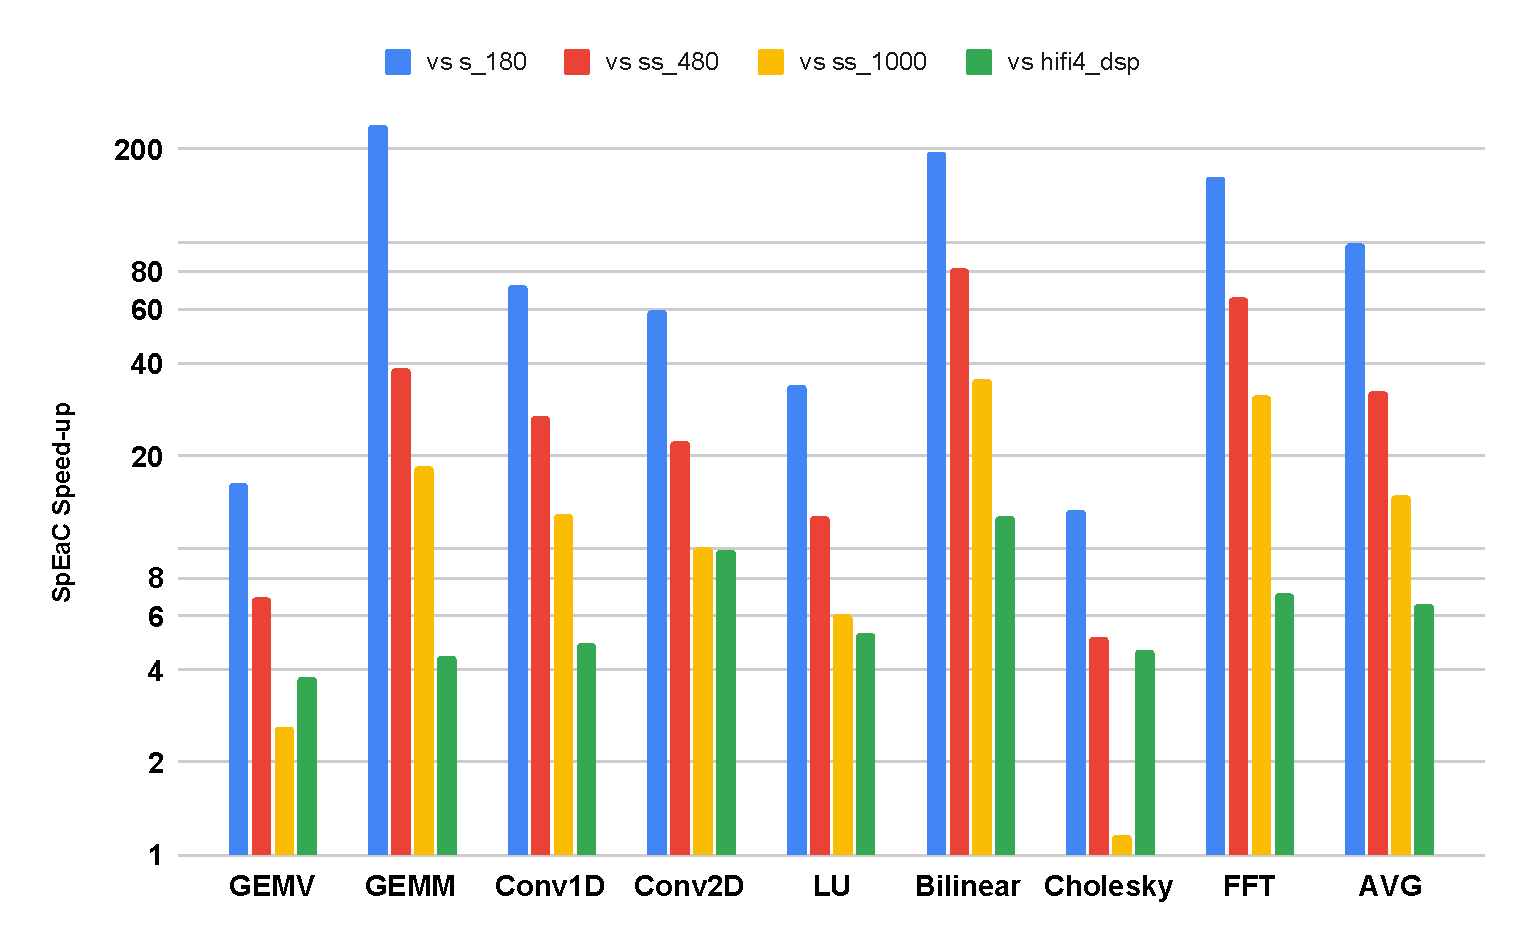
\includegraphics[width=\linewidth]{./figs/speedup.pdf}
    \caption{\small
    Speed-up of SpEaC over modeled cores.
    }
    \label{fig:earable_results}
\end{wrapfigure}

\begin{wrapfigure}{L}{0.5\textwidth}
    \centering
    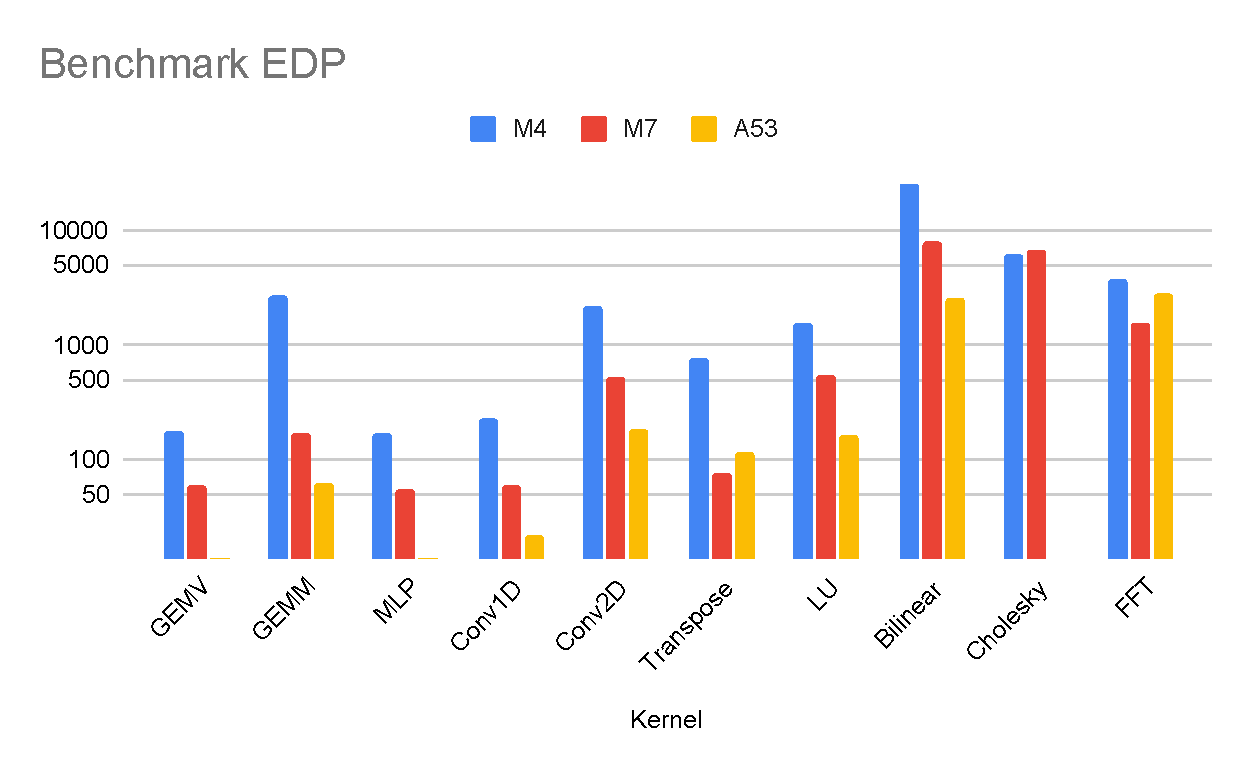
\includegraphics[width=\linewidth]{./figs/edp.pdf}
    \caption{\small
    Energy improvement from SpEaC over modeled cores.
    }
    \label{fig:earable_edp}
\end{wrapfigure}

Fig.~\ref{fig:earable_edp} shows the energy benefit of SpEaC relative to the
baseline cores. The benefits are up to \(160\times\) compared against the
microprocessors, and up to over \(42\times\) compared to the DSP.

The percentage of total energy consumption consumed by adders and multiplier
functional units is < 20\% for each kernel. The high overhead of control and
data movement reinforce the importance of minimizing the CGRA network costs
(using a tree, for example), the use of specialized FUs (using only fixed point
adders and multipliers on the substrate, for example), and the associated
memory system. Using kernel speed-up values from simulation, and with the
kernel-breakdown of Fig.~\ref{fig:earable_results}, we estimate the application
level speed-up and energy benefits of SpEaC. Compared against ss\_1000,
significant application level speed-ups are significant: \(3.3\times\) for
Deep- Speech and Ambisonic, \(6.6\times\) to \(9.6\times\) for HRTF audio,
\(3.6\) for the ResNet, \(2.2\times\) for ALBERT, \(6.4\times\) for DeepECGCNN,
and \(8.3\times\) for WaveToLetter. In fact, these speed-ups are achieved
despite ss\_1000 consuming \(2\times\) to \(2.5\times\) more power than SpEaC.
These speed-ups are large enough to allow SpEaC to meet the application-level
requirements of all applications, except ALBERT and EKF. Recall
that s\_180, ss\_480, and ss\_1000 met requirements for 0, 2, and 6 applications
respecitively.

To understand the system-level impact of SpEaC, we also consider non-compute
components. Table 5 lists power and latency of several non-compute components.
The latency overhead of the non-compute components is much smaller than the
estimated latency of Earbench applications on SpEaC. We estimate that, compared
to s\_180, ss\_480 and ss\_1000, the speedup of SpEaC on-average across all
EarBench applications is only reduced by 0.67\%, 0.51\% and 0.33\% respectively,
when the latency of all the non-compute components in Table 5 is added. We
similarly estimated (Figure 6) the number of times different EarBench
applications whose performance requirements are met by the SpEaC can be run on
the SpEaC given the energy budget of a \SI{45.4}{\milli\ampere\hour},
\SI{3.7}{\volt} battery.


\begin{wrapfigure}{L}{0.5\textwidth}
    \centering
    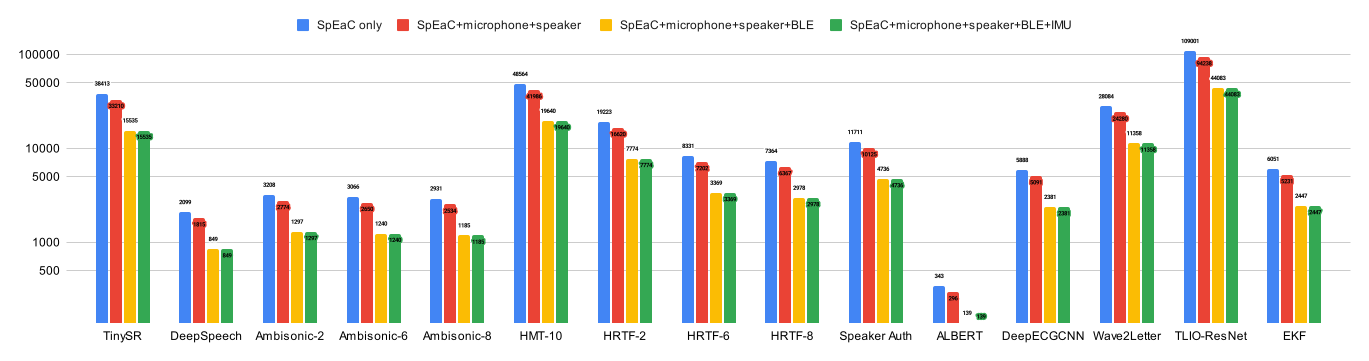
\includegraphics[width=\linewidth]{./figs/speakandsensors.png}
    \caption{\small
    Number of runs on SpEaC on a \SI{45.4}{\milli\ampere\hour}, \SI{3.7}{\volt}
    battery.
    }
    \label{fig:earable_edp}
\end{wrapfigure}

Our results show that even when the microphone, speaker, BLE and IMU sensor are
simultaneously consuming battery energy, the EarBench applications can still
run hundreds of times. E.g. DeepSpeech on 5s audio can run 849 times before
battery needs recharging; this corresponds to large-vocabulary speech
recognition for 1.14 hours. To validate our estimates, we ported TinySR to
SpEaC, implementing the FFT component on the CGRA. Based on TinySR’s estimates,
we had expected to see a \(2.7\times\) speed-up on SpEaC. Simulation of the SpEaC port
of TinySR showed a \(2.5\times\) speed-up, a −7\% error versus our analytic estimate. A
\(2.5\times\) performance improvement on TinySR also corresponds to a
\(5.8\times\) improvement in energy efficiency, and a \(14.4\times\)
improvement in EDP.


